\section{Data Flow Diagram}
\noindent Per Data Flow Diagram si intende uno schema in cui i blocchi rappresentano le varie operazioni, mentre le frecce descrivono il flusso dei dati. In questo caso, esso illustra come sono state distribuite le risorse, definite nella specifica, per unità di butterfly. Nel diagramma presentato di seguito, con un rettangolino nero si indica che il dato è salvato in un certo registro, l'asse verticale è quello temporale e presenta fino a dodici colpi di clock.

\begin{figure}[H]
      \centering
      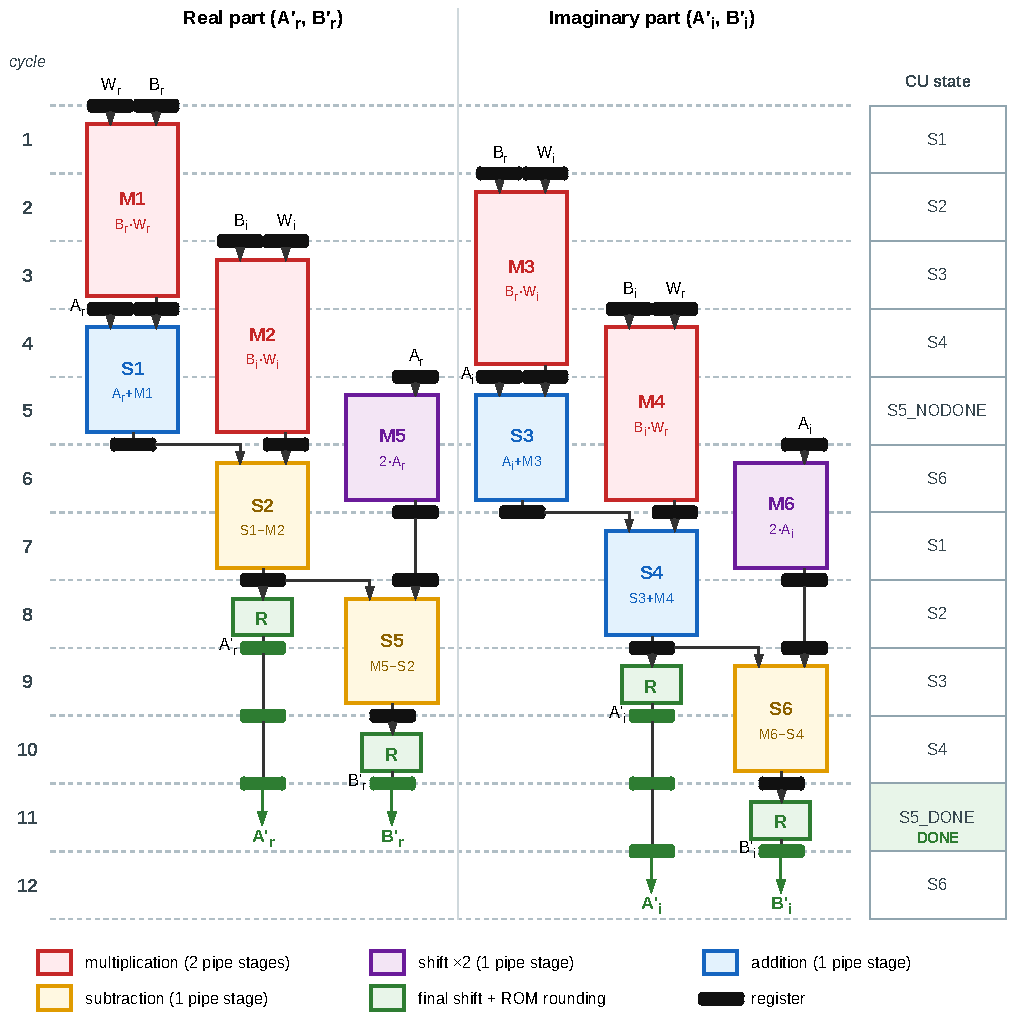
\includegraphics[width=1\textwidth]{fig01_dfd_butterfly}
      \caption{Data Flow Diagram dell'unità butterfly}
\end{figure} 

\noindent L'algoritmo da implementare prevede che l'unità compia le seguenti operazioni:
\begin{align*}
    A' &= A + B \cdot W^k \\
    B' &= A - B \cdot W^{(k+N/2)}
\end{align*}

\noindent dove A', B', A, B e i $W$ sono in generale dei numeri complessi. 
\noindent Da specifiche, all'interno di una singola butterfly, si hanno a disposizione un solo sommatore e un solo sottrattore, entrambi con uno stadio di pipe e un unico blocco che, a seconda di un segnale di controllo, può compiere una moltiplicazione caratterizzata da due stadi di pipe, oppure uno shift aritmetico verso sinistra dell'ingresso di una locazione (con uno stadio di pipe). Tutti questi blocchi svolgono operazioni su numeri reali. Perciò, è necessario scomporre le variabili nella loro parte Reale ($r$) e Immaginaria ($i$), e lavorare su queste. Al fine di ottenere i 4 risultati voluti $A'_r$,  $B'_r$, $A'_i$, $B'_i$ (ovvero le parti reali e immaginarie degli ingressi e delle uscite), è necessario svolgere 4 moltiplicazioni ($M_1$, $M_2$, $M_3$ e $M_4$), 2 shift aritmetici ($M_5$ e $M_6$), 3 somme ($S_1$,$S_3$ e $S_4$) e 3 sottrazioni ($S_2$, $S_5$ e $S_6$).

\begin{comment}
\begin{itemize}
    \item \textbf{Prodotto Complesso} ($P = B \cdot W$):
    \begin{itemize}
        \item $P_r = B_r W_r - B_i W_i$
        \item $P_i = B_r W_i + B_i W_r$.
     Richiede quattro moltiplicazioni, una sottrazione e una somma.
    \end{itemize}
    
    \item \textbf{Somma/Sottrazione Butterfly}:
    \begin{itemize}
        \item $A'_r = A_r + P_r, \quad A'_i = A_i + P_i$
        \item $B'_r = A_r - P_r, \quad B'_i = A_i - P_i$. Richiede due somme e due sottrazioni.
    \end{itemize}
\end{itemize}
\end{comment}

\noindent Avendo a disposizione un solo moltiplicatore/shifter fisico, le operazioni che lo necessitano devono essere serializzate. Il diagramma mostra sei utilizzi di tale blocco per ciascuna esecuzione della butterfly, indicati come segue:

\begin{itemize}
    \item Ciclo 1: si inizia l'esecuzione del calcolo $M_1 = B_{r} \quad \cdot \quad W_{r}$
    \item Ciclo 2: si inizia l'esecuzione del calcolo $M_3 = B_{r} \quad \cdot \quad W_{i}$
    \item Ciclo 3: si inizia l'esecuzione del calcolo $M_2 = B_{i} \quad \cdot \quad W_{i}$
    \item Ciclo 4: si inizia l'esecuzione del calcolo $M_4 = B_{i} \quad \cdot \quad W_{r}$
    \item Ciclo 5: si opera su $A_{r}$, moltiplicandolo per un fattore 2 mediante uno shift verso sinistra, iniziando il calcolo di $M_5$
    \item Ciclo 6: si opera su $A_{i}$, moltiplicandolo per un fattore 2 mediante uno shift verso sinistra, iniziando il calcolo di $M_6$
\end{itemize}
Invece, di seguito, si presentano le operazioni effettuate dal sommatore e dal sottrattore e in quale colpo di clock esse iniziano ad essere eseguite, specificando che i risultati di $S_2$, $S_4$, $S_5$, e $S_6$, a seguito di un opportuno arrotondamento, corrispondono alle uscite volute della butterfly $A'_r$, $A'_i$, $B'_r$ e $B'_i$.
\begin{itemize}
    \item Ciclo 4: si esegue il calcolo $S_{1} \quad = \quad A_{r} \quad + \quad M_1$
    \item Ciclo 5: si esegue il calcolo $S_{3} \quad = \quad A_{i} \quad + \quad M_3$
    \item Ciclo 6: si esegue il calcolo $S_{2} \quad = \quad S_{1}\quad - \quad M_2  \quad (= A'_{r}\ )$
    \item Ciclo 7: si esegue il calcolo $S_{4} \quad = \quad S_{3} \quad + \quad M_4  \quad (= A'_{i}\ )$
    \item Ciclo 8: si esegue il calcolo $S_{5}\quad = \quad M_5 \quad - \quad S_{2}  \quad (= B'_{r}\ )$
    \item Ciclo 9: si esegue il calcolo $S_{6}\quad = \quad M_6 \quad - \quad S_{4}  \quad (= B'_{i}\ )$
\end{itemize}
 
\noindent Infine, i blocchi verdi presenti nel DFD corrispondono allo stadio di "rounding": sono collocati alla fine di ogni catena di calcolo per riportare i risultati a 24 bit prima di fornirli in uscita. Come indicato nelle specifiche, l'arrotondamento richiede un ulteriore ciclo di clock per generare il valore finale, poiché il risultato approssimato deve essere salvato in un registro.

\noindent Il Data Flow Diagram proposto è una soluzione che si avvicina maggiormente alla tipologia ASAP ("As Soon As Possible"), obbligata dalla possibilità di utilizzo di un singolo moltiplicatore e dalla richiesta di andare il più veloce possibile.
Inoltre, anche le altre operazioni avvengono tutte il prima possibile, poiché, appena sono disponibili tutti gli operandi, si inizia una nuova operazione.

\noindent Si evidenzia, inoltre, che, dal settimo colpo di clock, il moltiplicatore non deve più eseguire nuove operazioni della butterfly appena considerata e non è più necessario mantenere salvati gli ingressi: l'unità può quindi iniziare nuovamente con il prodotto $M_1$ del nuovo set di dati. Di conseguenza, la singola elaborazione degli ingressi da parte del PE impiega dodici colpi di clock per completare tutte le operazioni e fornire in uscita tutti i risultati, ma l'unità può ricevere in ingresso nuovi dati ogni sei cicli. Quanto descritto è ciò che accade nel caso in cui si utilizzi l'unità in modalità continua,  come descritto nelle sezioni successive.
\begin{figure}[H]
      \centering
      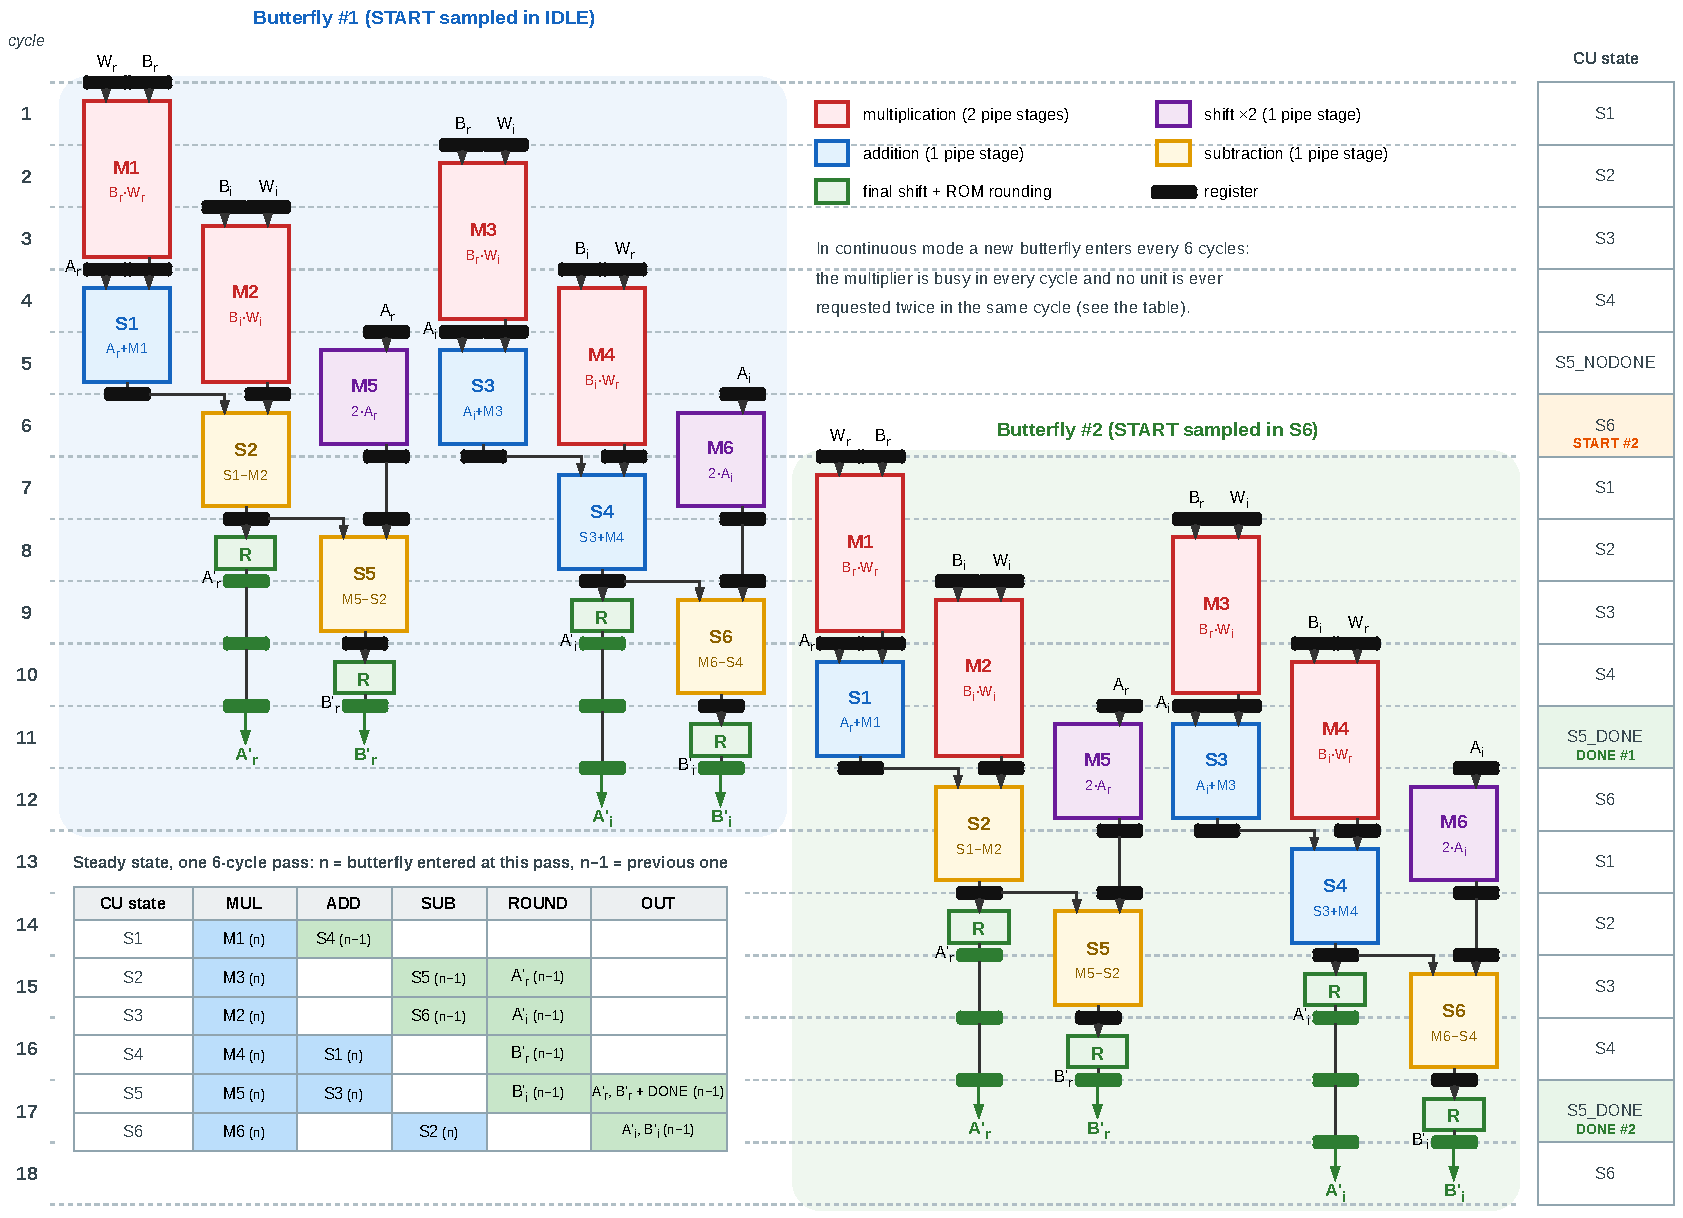
\includegraphics[width=1\textwidth]{fig02_dfd_continuous}
      \caption{Data Flow Diagram dell'unità butterfly in continua}
\end{figure}
